%! Author = gramic
%! Date = 26.04.24

% Preamble
\subsection{Patroni}
\label{subsec:evaluation_installation_patroni}
\subsubsection{Prerequisites}
Ganz am Anfang steht die Firewall.\\
Die Rules müssen auf \texttt{sks1232}, \texttt{sks1233}, \texttt{sks1234} und \texttt{sks9016} gesetzt werden:
\lstset{style=gra_codestyle}
\begin{lstlisting}[language=bash, caption=Patroni - Firewall Settings,captionpos=b,label={lst:patroni-firewall-settings},breaklines=true]
# sks1232 / sks1233 / sks1234 / sks9016(10.0.28.16)
nano /etc/iptables/rules.v4
*filter
:INPUT ACCEPT [0:0]
:FORWARD ACCEPT [0:0]
:OUTPUT ACCEPT [0:0]
-A INPUT -s 10.0.0.0/8 -p tcp -m tcp --dport 22 -j ACCEPT
-A INPUT -s 10.0.9.115/32 -p udp -m udp --dport 161 -m comment --comment "Allow SNMP for probe 10.0.9.115" -j ACCEPT
-A INPUT -s 10.0.9.76/32 -p udp -m udp --dport 161 -m comment --comment "Allow SNMP for probe 10.0.9.76" -j ACCEPT
-A INPUT -s 10.0.36.147/32 -p udp -m udp --dport 161 -m comment --comment "Allow SNMP for probe 10.0.36.147" -j ACCEPT
-A INPUT -s 10.0.9.35/32 -p udp -m udp --dport 161 -m comment --comment "Allow SNMP for probe 10.0.9.35" -j ACCEPT
-A INPUT -s 10.0.9.37/32 -p udp -m udp --dport 161 -m comment --comment "Allow SNMP for probe 10.0.9.37" -j ACCEPT
-A INPUT -s 10.0.9.74/32 -p udp -m udp --dport 161 -m comment --comment "Allow SNMP for probe 10.0.9.74" -j ACCEPT
-A INPUT -s 10.0.9.75/32 -p udp -m udp --dport 161 -m comment --comment "Allow SNMP for probe 10.0.9.75" -j ACCEPT
-A INPUT -s 10.0.9.36/32 -p udp -m udp --dport 161 -m comment --comment "Allow SNMP for probe 10.0.9.36" -j ACCEPT
-A INPUT -s 10.0.9.14/32 -p udp -m udp --dport 161 -m comment --comment "Allow SNMP for probe 10.0.9.14" -j ACCEPT
-A INPUT -s 10.0.0.0/8 -p icmp -m icmp --icmp-type 8 -j ACCEPT
# generell
-A INPUT -s 10.0.0.0/8 -p tcp -m tcp --dport 443 -j ACCEPT
# postgres
-A INPUT -s 10.0.0.0/8 -p tcp -m tcp --dport 5432 -j ACCEPT
# patroni
-A INPUT -s 10.0.0.0/8 -p tcp -m tcp --dport 2379 -j ACCEPT
-A INPUT -s 10.0.0.0/8 -p tcp -m tcp --dport 2380 -j ACCEPT
-A INPUT -s 10.0.0.0/8 -p tcp -m tcp --dport 2376 -j ACCEPT
-A INPUT -s 10.0.0.0/8 -p tcp -m tcp --dport 6432 -j ACCEPT
-A INPUT -s 10.0.0.0/8 -p tcp -m tcp --dport 8008 -j ACCEPT
-A INPUT -s 10.0.0.0/8 -p tcp -m tcp --dport 7000 -j ACCEPT
-A INPUT -s 10.0.0.0/8 -p tcp -m tcp --dport 8080 -j ACCEPT
COMMIT
# Completed

systemctl restart iptables
systemctl status iptables
\end{lstlisting}

Danach muss der Proxy gesetzt werden:
\lstset{style=gra_codestyle}
\begin{lstlisting}[language=bash, caption=Patroni - Proxy Settings,captionpos=b,label={lst:patroni-proxy-settings},breaklines=true]
# sks1232 / sks1233 / sks1234
# Proxy setzen
# nano /etc/profile.d/proxy.sh
export https_proxy=http://sproxy.sivc.first-it.ch:8080
export HTTPS_PROXY=http://sproxy.sivc.first-it.ch:8080
export http_proxy=http://sproxy.sivc.first-it.ch:8080
export HTTP_PROXY=http://sproxy.sivc.first-it.ch:8080
export no_proxy=localhost,127.0.0.0/8,::1,10.0.0.0/8,172.16.0.0/12,192.168.0.0/16
export NO_PROXY=localhost,127.0.0.0/8,::1,10.0.0.0/8,172.16.0.0/12,192.168.0.0/16
# source /etc/profile.d/proxy.sh
\end{lstlisting}

Damit das PostgreSQL-Repository eingebunden werden kann,\\
muss dem apt-Proxy gesetzt werden.\\
Da via \Gls{Foreman} installiert wurde, muss dieser ausgenommen werden:
\lstset{style=gra_codestyle}
\begin{lstlisting}[language=bash, caption=Patroni - apt-Proxy Settings,captionpos=b,label={lst:patroni-apt-proxy-settings},breaklines=true]
# sks1232 / sks1233 / sks1234
# apt-Proxy setzen
# nano /etc/apt/apt.conf.d/proxy.conf
Acauire::http::Proxy "http://sproxy.sivc.first-it.ch:8080";
Acauire::https::Proxy "http://sproxy.sivc.first-it.ch:8080";
Acquire::http::proxy::foreman.ksgr.ch "DIRECT";
\end{lstlisting}

Im nächsten Schritt kann das PostgreSQL-Repository eingebunden werden.
\begin{warning}
Achtung, die von PostgreSQL beschriebene Variante wurde in Debian 10 als Deprecated gesetzt,
mit Debian 13 wird diese Repository-Integration zu einem Fehler werden.
\end{warning}

\lstset{style=gra_codestyle}
\begin{lstlisting}[language=bash, caption=Patroni - PostgreSQL einbinden,captionpos=b,label={lst:patroni-include-repository},breaklines=true]
# sks1232 / sks1233 / sks1234
# PostgreSQL Repository einbinden
sudo sh -c 'echo "deb https://apt.postgresql.org/pub/repos/apt $(lsb_release -cs)-pgdg main" > /etc/apt/sources.list.d/pgdg.list'
wget --quiet -O - https://www.postgresql.org/media/keys/ACCC4CF8.asc | sudo apt-key add -

# Ausloggen und wieder einloggen
apt update
\end{lstlisting}

Nun muss der \Gls{PostgreSQL Cluster}, Patroni, python3-etcd und python3-psycopg2 installiert werden:
\lstset{style=gra_codestyle}
\begin{lstlisting}[language=bash, caption=Patroni - Prerequisites installieren,captionpos=b,label={lst:patroni-prerequisites-install},breaklines=true]
apt install postgresql-16 postgresql-server-dev-16 patroni python3-etcd python3-psycopg2
\end{lstlisting}

Im nächsten Schritt müssen Patroni und der \Gls{PostgreSQL Cluster} gestoppt werden:
\lstset{style=gra_codestyle}
\begin{lstlisting}[language=bash, caption=Patroni - Stop Patroni und PostgreSQL,captionpos=b,label={lst:patroni-stop-postgresql-patroni},breaklines=true]
systemctl stop postgresql patroni
\end{lstlisting}

Anschliessend muss noch vom PostgreSQL-Verzeichnis \texttt{/usr/lib/postgresql/16/bin/} ein Symlink nach \texttt{/usr/sbin/} gesetzt werden:
\lstset{style=gra_codestyle}
\begin{lstlisting}[language=bash, caption=Patroni - Symlink binaries,captionpos=b,label={lst:patroni_symlink_bins},breaklines=true]
ln -s /usr/lib/postgresql/16/bin/* /usr/sbin/
\end{lstlisting}

Zu guter Letzt sollte geprüft werden, ob alle Versionen passen und am richtigen Ort sind:
\lstset{style=gra_codestyle}
\begin{lstlisting}[language=bash, caption=Patroni - Checks,captionpos=b,label={lst:patroni-checks},breaklines=true]
which patroni
which psql
patroni --version
\end{lstlisting}
Damit kann zum \gls{etcd} übergegangen werden.
\subsubsection{Installation etcd}
Auf \texttt{sks9016} sollte erst das Repository angepasst werden und anschliessend der \texttt{etcd-server} installiert werden:
\lstset{style=gra_codestyle}
\begin{lstlisting}[language=bash, caption=etcd - Installation,captionpos=b,label={lst:etcd_install},breaklines=true]
apt update
apt install etcd-server
\end{lstlisting}

Die Konfiguration ist simpel.\\
Die IP muss gesetzt werden, ein Listener auf Localhost und IP gesetzt werden:
\lstset{style=gra_codestyle}
\begin{lstlisting}[language=bash, caption=etcd - Konfiguration,captionpos=b,label={lst:etcd_configuration},breaklines=true]
# nano /etc/default/etcd
ETCD_LISTEN_PEER_URLS="http://10.0.28.16:2380"
ETCD_LISTEN_CLIENT_URLS="http://localhost:2379,http://10.0.28.16:2379"
ETCD_INITIAL_ADVERTISE_PEER_URLS="http://10.0.28.16:2380"
ETCD_INITIAL_CLUSTER="default=http://10.0.28.16:2380,"
ETCD_ADVERTISE_CLIENT_URLS="http://10.0.28.16:2379"
ETCD_INITIAL_CLUSTER_TOKEN="etcd-cluster"
ETCD_INITIAL_CLUSTER_STATE="new"
\end{lstlisting}

Der Service sollte neu gestartet und seine Lauffähigkeit getestet werden:
\lstset{style=gra_codestyle}
\begin{lstlisting}[language=bash, caption=etcd - restart,captionpos=b,label={lst:etcd_restart},breaklines=true]
systemctl restart etcd
systemctl is-enabled etcd
systemctl status etcd
\end{lstlisting}

Es sollte nun ein Member gelistet werden:
\lstset{style=gra_codestyle}
\begin{lstlisting}[language=bash, caption=etcd - member list,captionpos=b,label={lst:etcd_member_list},breaklines=true]
etcdctl member list
\end{lstlisting}

Damit kann nun das Bootstrapping gestartet werden.

\subsubsection{Bootstrapping}
Zuerst müssen die yml-Konfigurationen gesetzt werden.\\
Am besten wird das bestehende File jeweils gelöscht:
\lstset{style=gra_codestyle}
\begin{lstlisting}[language=bash, caption=Patroni Bootstrap - Konfiguration bereinigen,captionpos=b,label={lst:patroni-bootstrap-cleanup-yml},breaklines=true]
rm /etc/patroni/config.yml
nano /etc/patroni/config.yml
\end{lstlisting}

Die yml-Files sehen wie folgt aus:
\lstset{style=gra_codestyle}
\begin{lstlisting}[language=yaml, caption=Patroni - Konfiguration - sks1232,captionpos=b,label={lst:sks1232_patroni.yml},breaklines=true]
# Scope of PostgreSQL
scope: postgres
# Namespace for the PostgreSQL database
namespace: /db/
# Name of the PostgreSQL instance
name: postgres01
# Patroni REST API Configuration
restapi:
    # The IP address and port on which the REST API should listen
    listen: 10.0.20.110:8008

    # The IP address and port to which clients should connect
    connect_address: 10.0.20.110:8008
# Patroni Etcd Configuration
etcd3:
    # The host address and port of the Etcd server
    host: 10.0.28.16:2379
# Patroni Bootstrap Configuration
bootstrap:
    # Configuration parameters for distributed configuration store (DCS)
    dcs:
        ttl: 30
        loop_wait: 10
        retry_timeout: 10
        maximum_lag_on_failover: 1048576
        postgresql:
            # Use pg_rewind during bootstrap
            use_pg_rewind: true
            #   Change pg_wal
            create_replica_methods:
                - basebackup
            basebackup:
                max-rate: '100M'
                waldir: "/srv/data/pg_wal"
    # Initdb configuration
    # Initdb configuration
    initdb:
        - auth: scram-sha-256
        - encoding: UTF8
        - data-checksums
    # pg_hba.conf entries for replication and general access
    pg_hba:
        - host replication replicator 127.0.0.1/32 scram-sha-256
        - host replication replicator 10.0.20.110/0 scram-sha-256
        - host replication replicator 10.0.20.111/0 scram-sha-256
        - host replication replicator 10.0.20.112/0 scram-sha-256
        - host all all 0.0.0.0/0 scram-sha-256
    # Adding default user admin with password admin
    users:
      admin:
          password: admin
          options:
              - createrole
              - createdb
# Patroni PostgreSQL Configuration
postgresql:
    # PostgreSQL server listening address and port
    listen: 10.0.20.110:5432
    # Connect address for PostgreSQL clients
    connect_address: 10.0.20.110:5432
    # Data directory for PostgreSQL
    data_dir: /var/lib/patroni
    # Path to the pgpass file
    pgpass: /tmp/pgpass
    # Authentication configuration
    authentication:
        # Replication of user credentials
        replication:
            username: replicator
            password: replicator
        # Superuser credentials
        superuser:
            username: postgres
            password: postgres
    # Additional PostgreSQL parameters
    parameters:

        # Directory for Unix socket
        unix_socket_directories: '.'
        # Password encryption method
        password_encryption: 'scram-sha-256'
# Patroni Tags Configuration
tags:
    # Prevents a node from being promoted in case of failure
    nofailover: false
    # Prevents the load balancer from considering this node
    noloadbalance: false
    # Prevents a replica from being created by cloning
    clonefrom: false
    # Prevents synchronous replication from being enforced
    nosync: false

\end{lstlisting}

\lstset{style=gra_codestyle}
\begin{lstlisting}[language=yaml, caption=Patroni - Konfiguration - sks1233,captionpos=b,label={lst:sks1233_patroni.yml},breaklines=true]
# Scope of PostgreSQL
scope: postgres
# Namespace for the PostgreSQL database
namespace: /db/
# Name of the PostgreSQL instance
name: postgres02
# Patroni REST API Configuration
restapi:
    # The IP address and port on which the REST API should listen
    listen: 10.0.20.111:8008

    # The IP address and port to which clients should connect
    connect_address: 10.0.20.111:8008
# Patroni Etcd Configuration
etcd3:
    # The host address and port of the Etcd server
    host: 10.0.28.16:2379
# Patroni Bootstrap Configuration
bootstrap:
    # Configuration parameters for distributed configuration store (DCS)
    dcs:
        ttl: 30
        loop_wait: 10
        retry_timeout: 10
        maximum_lag_on_failover: 1048576
        postgresql:
            # Use pg_rewind during bootstrap
            use_pg_rewind: true
            #   Change pg_wal
            create_replica_methods:
                - basebackup
            basebackup:
                max-rate: '100M'
                waldir: "/srv/data/pg_wal"
    # Initdb configuration
    # Initdb configuration
    initdb:
        - auth: scram-sha-256
        - encoding: UTF8
        - data-checksums
    # pg_hba.conf entries for replication and general access
    pg_hba:
        - host replication replicator 127.0.0.1/32 scram-sha-256
        - host replication replicator 10.0.20.110/0 scram-sha-256
        - host replication replicator 10.0.20.111/0 scram-sha-256
        - host replication replicator 10.0.20.112/0 scram-sha-256
        - host all all 0.0.0.0/0 scram-sha-256
    # Adding default user admin with password admin
    users:
      admin:
          password: admin
          options:
              - createrole
              - createdb
# Patroni PostgreSQL Configuration
postgresql:
    # PostgreSQL server listening address and port
    listen: 10.0.20.111:5432
    # Connect address for PostgreSQL clients
    connect_address: 10.0.20.111:5432
    # Data directory for PostgreSQL
    data_dir: /var/lib/patroni
    # Path to the pgpass file
    pgpass: /tmp/pgpass

    # Authentication configuration
    authentication:
        # Replication of user credentials
        replication:
            username: replicator
            password: replicator
        # Superuser credentials
        superuser:
            username: postgres
            password: postgres
    # Additional PostgreSQL parameters
    parameters:
        # Directory for Unix socket
        unix_socket_directories: '.'
        # Password encryption method
        password_encryption: 'scram-sha-256'
# Patroni Tags Configuration
tags:
    # Prevents a node from being promoted in case of failure
    nofailover: false
    # Prevents the load balancer from considering this node
    noloadbalance: false
    # Prevents a replica from being created by cloning
    clonefrom: false
    # Prevents synchronous replication from being enforced
    nosync: false

\end{lstlisting}

\lstset{style=gra_codestyle}
\begin{lstlisting}[language=yaml, caption=Patroni - Konfiguration - sks1234,captionpos=b,label={lst:sks1234_patroni.yml},breaklines=true]
# Scope of PostgreSQL
scope: postgres
# Namespace for the PostgreSQL database
namespace: /db/
# Name of the PostgreSQL instance
name: postgres03
# Patroni REST API Configuration
restapi:
    # The IP address and port on which the REST API should listen
    listen: 10.0.20.112:8008

    # The IP address and port to which clients should connect
    connect_address: 10.0.20.112:8008
# Patroni Etcd Configuration
etcd3:
    # The host address and port of the Etcd server
    host: 10.0.28.16:2379
# Patroni Bootstrap Configuration
bootstrap:
    # Configuration parameters for distributed configuration store (DCS)
    dcs:
        ttl: 30
        loop_wait: 10
        retry_timeout: 10
        maximum_lag_on_failover: 1048576
        postgresql:
            # Use pg_rewind during bootstrap
            use_pg_rewind: true
            #   Change pg_wal
            create_replica_methods:
                - basebackup
            basebackup:
                max-rate: '100M'
                waldir: "/srv/data/pg_wal"
    # Initdb configuration
    initdb:
        - auth: scram-sha-256
        - encoding: UTF8
        - data-checksums
    # pg_hba.conf entries for replication and general access
    pg_hba:
        - host replication replicator 127.0.0.1/32 scram-sha-256
        - host replication replicator 10.0.20.110/0 scram-sha-256
        - host replication replicator 10.0.20.111/0 scram-sha-256
        - host replication replicator 10.0.20.112/0 scram-sha-256
        - host all all 0.0.0.0/0 scram-sha-256
    # Adding default user admin with password admin
    users:
      admin:
          password: admin
          options:
              - createrole
              - createdb
# Patroni PostgreSQL Configuration
postgresql:
    # PostgreSQL server listening address and port
    listen: 10.0.20.112:5432
    # Connect address for PostgreSQL clients
    connect_address: 10.0.20.112:5432
    # Data directory for PostgreSQL
    data_dir: /var/lib/patroni
    # Path to the pgpass file
    pgpass: /tmp/pgpass
    # Authentication configuration
    authentication:
        # Replication of user credentials
        replication:
            username: replicator
            password: replicator
        # Superuser credentials
        superuser:
            username: postgres
            password: postgres
    # Additional PostgreSQL parameters
    parameters:
        unix_socket_directories: '.'
        # Password encryption method
        password_encryption: 'scram-sha-256'
# Patroni Tags Configuration
tags:
    # Prevents a node from being promoted in case of failure
    nofailover: false
    # Prevents the load balancer from considering this node
    noloadbalance: false
    # Prevents a replica from being created by cloning
    clonefrom: false
    # Prevents synchronous replication from being enforced
    nosync: false

\end{lstlisting}

Sehr wichtig ist, dass das \texttt{pg\_hba.conf}-File mitgegeben wird.\\
Ansonsten kann nicht auf die Datenbank zugegriffen werden.\\
Für den User \texttt{replication} müssen die IP-Adressen aller Nodes gesetzt werden.\\
Im Evaluations-Enviroment soll zudem der Zugriff von überall mit Passwort möglich sein.\\
Dies wird mit der letzten Zeile ermöglicht:
\lstset{style=gra_codestyle}
\begin{lstlisting}[language=bash, caption=Patroni Bootstrap - pg\_hba,captionpos=b,label={lst:patroni-pg_hba},breaklines=true]
host replication replicator 127.0.0.1/32 scram-sha-256
host replication replicator 10.0.20.110/0 scram-sha-256
host replication replicator 10.0.20.111/0 scram-sha-256
host replication replicator 10.0.20.112/0 scram-sha-256
host all all 0.0.0.0/0 scram-sha-256
\end{lstlisting}

Nun muss das Verzeichnis für PostgreSQL im Patroni-Verzeichnis erstellt und berechtigt werden:
\lstset{style=gra_codestyle}
\begin{lstlisting}[language=bash, caption=Patroni Bootstrap - Patroni-Verzeichnis,captionpos=b,label={lst:patroni-directory},breaklines=true]
mkdir -p /var/lib/patroni
chown -R postgres:postgres /var/lib/patroni
chmod 700 /var/lib/patroni
\end{lstlisting}

Jetzt können die Dienste auf den Patroni-Servern neu gestartet werden, Patroni sollte nun lauffähig sein:
\lstset{style=gra_codestyle}
\begin{lstlisting}[language=bash, caption=Patroni Bootstrap - Neu starten,captionpos=b,label={lst:patroni-restart},breaklines=true]
systemctl start patroni
systemctl status patroni
patronictl -c /etc/patroni/config.yml list
\end{lstlisting}

Wenn es lauffähig ist, muss noch aufgeräumt werden.\\
Der bestehende \Gls{PostgreSQL Cluster} muss disabled werden:
\lstset{style=gra_codestyle}
\begin{lstlisting}[language=bash, caption=Patroni Bootstrap - Disable PostgreSQL,captionpos=b,label={lst:patroni-disable-postgresql},breaklines=true]
sudo systemctl disable --now postgresql
\end{lstlisting}

\subsubsection{HAproxy}
Final kann nun HAproxy installiert werden.\\
Zuerst müssen die Hosts hinterlegt werden:
\lstset{style=gra_codestyle}
\begin{lstlisting}[language=bash, caption=HAproxy - Hostliste,captionpos=b,label={lst:haproxy_hostlist},breaklines=true]
#nano /etc/hosts
10.0.20.110    postgres01
10.0.20.111    postgres02
10.0.20.112    postgres03
\end{lstlisting}

Nun müssen die Repositories aktualisiert werden und HAproxy installiert werden:
\lstset{style=gra_codestyle}
\begin{lstlisting}[language=bash, caption=HAproxy - Installation,captionpos=b,label={lst:haproxy_installation},breaklines=true]
apt update
apt install haproxy
\end{lstlisting}

Mit der Installation kommt ein Konfig-File mit.\\
Das soll gesichert werden:
\lstset{style=gra_codestyle}
\begin{lstlisting}[language=bash, caption=HAproxy - Safe Alte Config,captionpos=b,label={lst:haproxy_safe_old_config},breaklines=true]
mv /etc/haproxy/haproxy.cfg /etc/haproxy/haproxy.cfg.orig
\end{lstlisting}

Nun muss die neue Konfiguration geschrieben werden:
\lstset{style=gra_codestyle}
\begin{lstlisting}[language=bash, caption=HAproxy - Konfiguration,captionpos=b,label={lst:haproxy_config},breaklines=true]
#nano /etc/haproxy/haproxy.cfg
# Global configuration settings
global
    # Maximum connections globally
    maxconn 100
    # Logging settings
    log 127.0.0.1 local2

# Default settings
defaults
    # Global log configuration
    log global
    # Set mode to TCP
    mode tcp
    # Number of retries
    retries 2
    # Client timeout
    timeout client 30m
    # Connect timeout
    timeout connect 4s
    # Server timeout
    timeout server 30m
    # Check timeout
    timeout check 5s

# Stats configuration
listen stats
    # Set mode to HTTP
    mode http
    # Bind to port 8080
    bind *:8080
    # Enable stats
    stats enable
    # Stats URI
    stats uri /

# PostgreSQL configuration
listen postgres
    # Bind to port 5432
    bind *:5432
    # Enable HTTP check
    option httpchk
    # Expect status 200
    http-check expect status 200
    # Server settings
    default-server inter 3s fall 3 rise 2 on-marked-down shutdown-sessions
    # Define PostgreSQL servers
    server postgres01 10.0.20.110:5432 maxconn 100 check port 8008
    server postgres02 10.0.20.111:5432 maxconn 100 check port 8008
    server postgres03 10.0.20.112:5432 maxconn 100 check port 8008
\end{lstlisting}

Nun kann HAproxy neu gestartet werden:
\lstset{style=gra_codestyle}
\begin{lstlisting}[language=bash, caption=HAproxy - Restart,captionpos=b,label={lst:haproxy_restart},breaklines=true]
systemctl restart haproxy
systemctl status haproxy
\end{lstlisting}

Nun kann HAproxy geöffnet werden:
\url{http://10.0.28.16:8080/}

Es sollte nun so aussehen:
\begin{figure}[H]
    \centering
    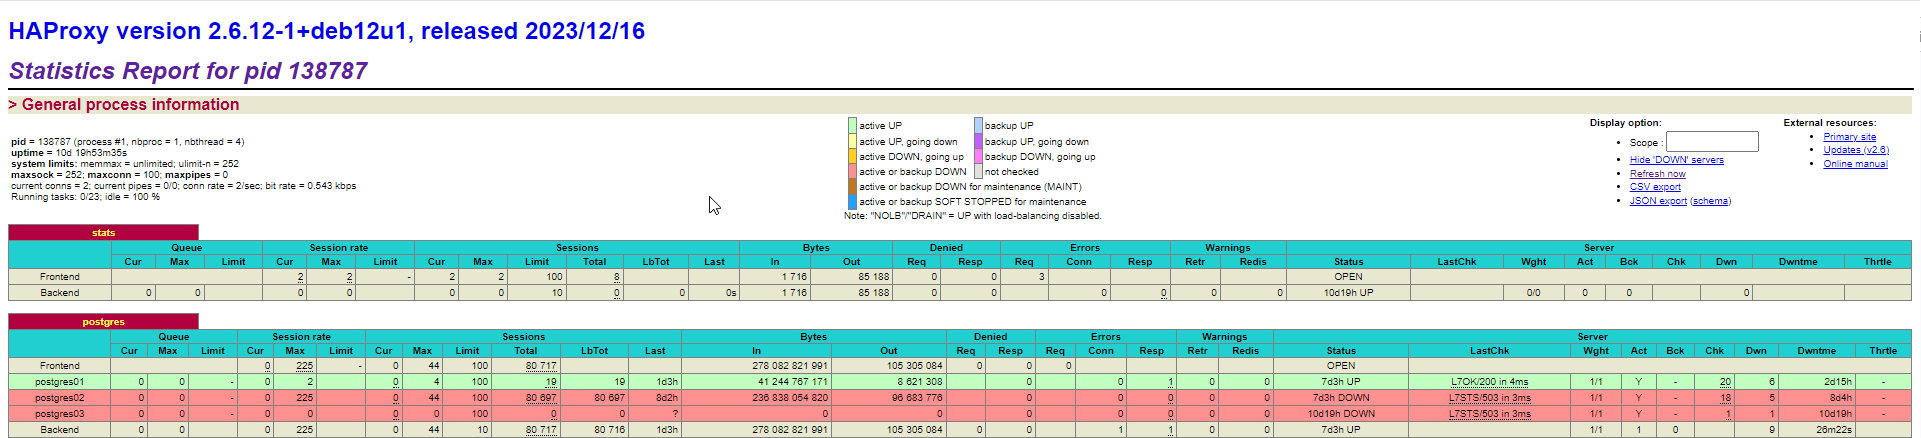
\includegraphics[width=0.8\linewidth]{source/implementation/evaluation/postgresql_ha_solutions/patroni/haproxy_webgui}
    \caption{HAproxy - Web-GUI}
    \label{fig:haproxy-webgui}
\end{figure}

\subsubsection{Rekonfiguration mit 250GiB Storage}
Sobald die neue Disk im \Gls{VMware vSphere} erfasst wurde, muss die Disk auf den Servern gemountet werden:
\lstset{style=gra_codestyle}
\begin{lstlisting}[language=bash, caption=Patroni - 250GiB Disk mount,captionpos=b,label={lst:patroni_250gib_disk_mount},breaklines=true]
echo "- - -" | tee /sys/class/scsi_host/host*/scan && lsblk

fdisk /dev/sdb
	n -> all default values
	t -> 8e
	p -> Kontrolle
	w

pvcreate /dev/sdb1 && \
vgcreate vgdata /dev/sdb1 && \
lvcreate -l 100%FREE -n lvdata vgdata && \
mkfs.ext4 /dev/vgdata/lvdata && \
mkdir -p /srv/data && \
cp /etc/fstab /tmp/fstab.bak && \
echo "/dev/vgdata/lvdata	/srv/data	ext4	defaults	0	0" >> /etc/fstab && \
systemctl daemon-reload && mount -a && lsblk
\end{lstlisting}

Nun können die Verzeichnisse angelegt werden.\\
Nebst dem Verzeichnis für die Indizes und Daten braucht es auch ein neues \texttt{pg\_wal}-Verzeichnis:
\lstset{style=gra_codestyle}
\begin{lstlisting}[language=bash, caption=Patroni - 250GiB Verzeichnisse,captionpos=b,label={lst:patroni_250gib_disk_directories},breaklines=true]
mkdir -p /srv/data/eval_index_tablespace
chown -R postgres:postgres /srv/data/eval_index_tablespace
chmod 700 /srv/data/eval_index_tablespace

mkdir -p /srv/data/eval_data_tablespace
chown -R postgres:postgres /srv/data/eval_data_tablespace
chmod 700 /srv/data/eval_data_tablespace

mkdir -p /srv/data/self_healing_test_index_tablespace
chown -R postgres:postgres /srv/data/self_healing_test_index_tablespace
chmod 700 /srv/data/self_healing_test_index_tablespace

mkdir -p /srv/data/self_healing_test_data_tablespace
chown -R postgres:postgres /srv/data/self_healing_test_data_tablespace
chmod 700 /srv/data/self_healing_test_data_tablespace

mkdir -p /srv/data/pg_wal
chown -R postgres:postgres /srv/data/pg_wal
chmod 700 /srv/data/pg_wal
\end{lstlisting}

Um das \texttt{WAL}-Verzeichnis umzuhängen, muss erst die der Patroni-Cluster gestoppt werden:
\lstset{style=gra_codestyle}
\begin{lstlisting}[language=bash, caption=Patroni - 250GiB Cluster Pause,captionpos=b,label={lst:patroni_250gib_cluster_stop},breaklines=true]
patronictl -c /etc/patroni/config.yml pause
\end{lstlisting}

Wichtig ist, dass auch PostgreSQL gestoppt ist.\\
Da die PostgreSQL Binaries nun im Patroni-Verzeichnis liegen und auch dort das Socket-File läuft,\\
muss das Verzeichnis zwingend als Daten-Verzeichnisparameter (\texttt{-D}) angegeben werden,\\
sonst wird es zu einem Socket-Fehler kommen.\\
Zwingend ist zudem, das Command als \texttt{postgres}-User auszuführen:
\lstset{style=gra_codestyle}
\begin{lstlisting}[language=bash, caption=Patroni - 250GiB PostgreSQL stoppen,captionpos=b,label={lst:patroni_250gib_stop_postgresql},breaklines=true]
sudo su - postgres
/usr/sbin/pg_ctl stop -D /var/lib/patroni/
\end{lstlisting}

Ganz wichtig ist nun, das ganze \texttt{pg\_wal}-Verzeichnis zu verschieben.\\
So das die \texttt{WAL}-Files kopiert werden.\\
Da ein symlink gezogen wird, muss das bestehende Verzeichnis garantiert gelöscht sein:
\lstset{style=gra_codestyle}
\begin{lstlisting}[language=bash, caption=Patroni - 250GiB move pg\_wal,captionpos=b,label={lst:patroni_250gib_move_pg_wal},breaklines=true]
mv /var/lib/patroni/pg_wal/* /srv/data/pg_wal
ln -s /srv/data/pg_wal /var/lib/patroni/pg_wal
ls -l /var/lib/patroni/pg_wal
\end{lstlisting}

Die Berechtigung muss anschliessend wieder mit root-Rechten gesetzt werden:
\lstset{style=gra_codestyle}
\begin{lstlisting}[language=bash, caption=Patroni - 250GiB chmod - chown pg\_wal,captionpos=b,label={lst:patroni_250gib_chmod_chown_pg_wal},breaklines=true]
chown -R postgres:postgres /var/lib/patroni/pg_wal
chmod 700 /var/lib/patroni/pg_wal
\end{lstlisting}

Jetzt muss erst PostgreSQL wieder gestartet werden.\\
Wenn alle Datenbanken auf allen Patroni-Nodes wieder lauffähig sind, kann der Cluster wieder aktiviert werden:
\lstset{style=gra_codestyle}
\begin{lstlisting}[language=bash, caption=Patroni - 250GiB PostgreSQL - Patroni resume,captionpos=b,label={lst:patroni_250gib_postgresql_patroni_resume},breaklines=true]
/usr/sbin/pg_ctl start -D /var/lib/patroni/
patronictl -c /etc/patroni/config.yml resume
\end{lstlisting}

Zum Schluss sollte noch zwingend geprüft werden, ob der Cluster funktionsfähig ist:
\lstset{style=gra_codestyle}
\begin{lstlisting}[language=bash, caption=Patroni - 250GiB Finaler Check,captionpos=b,label={lst:patroni_250gib_final_check},breaklines=true]
patronictl -c /etc/patroni/config.yml list
\end{lstlisting}

Wenn Patroni nun wieder einsatzfähig ist, müssen noch die optimierten Parameter gesetzt werden.\\
Folgende Parameter wurden gesetzt:\\
\begin{description}
    \item \textbf{max\_connections}\hfill \\Damit die 7000 Transaktionen sicher abgesetzt werden können.
    \item \textbf{superuser\_reserved\_connections}\hfill \\Mindestens 10 \texttt{postgres}-Verbindungen müssen gemacht werden können.
    \item \textbf{max\_worker\_processes}\hfill \\Damit genügend Worker vorhanden sind, um die \texttt{WAL}-Files abzuarbeiten, wurde deren Zahl auf 16 erhöht.
    \item \textbf{wal\_log\_hints}\hfill \\Stellt sicher, dass der gesamte Diskpage-Inhalt ins \texttt{WAL} geschrieben wird.
    \item \textbf{max\_wal\_senders}\hfill \\Um den Replikations-Throughput zu erhöhen, wurden 16 Sender aktiviert
    \item \textbf{max\_replication\_slots}\hfill \\Damit die 16 Sender auch auf der Gegenseite abgearbeitet werden,\\müssen die entsprechenden Slots bereitgestellt werden.
    \item \textbf{wal\_keep\_size}\hfill \\Damit die \texttt{WAL}-Files nicht zu gross werden und somit auch das Replication-Lag,\\wurde die Grösse auf 1 GiB reduziert.\\Das zwingt den Primary dazu, die \texttt{WAL}-Files nur bis zu maximal 1 GiB aufzubewahren, bevor sie archiviert werden.\\Das ist wichtig, wenn Diskspace nicht im Überfluss vorhanden ist.
    \item \textbf{wal\_level}\hfill \\Der Level wurde auf logical gesetzt, damit alle Informationen geschrieben werden.
    \item \textbf{wal\_buffers}\hfill \\Der Buffer wurde auf 16 MiB erhöht.
    \item \textbf{wal\_writer\_delay}\hfill \\Wenn der WAL-Writer einen Flush durchgeführt hat, geht er in ein Timeout.\\Dies wurde auf 20 ms heruntergesetzt, damit rasch wieder geschrieben wird.
    \item \textbf{wal\_writer\_flush\_after}\hfill \\Definiert, ab welcher Grösse der Cache des WAL-Writers auf die Disk geschrieben wird.\\Wurde auf 1 MiB gesetzt um rasch auf die Disk schreiben zu können.
    \item \textbf{min\_wal\_size}\hfill \\Damit die \texttt{WAL}-Files nicht zu schnell repliziert werden und die Standby-Server, aber auch der Primary-Server nicht überlastet werden,\\sollen die Files mindestens 1 GiB gross werden, bevor sie repliziert werden.
    \item \textbf{max\_wal\_size}\hfill \\Auf der anderen Seite soll trotzdem nicht zu lange gewartet werden,\\die maximale Grösse wurde auf 5 GiB begrenzt.
    \item \textbf{commit\_delay}\hfill \\Maximal 20 ms soll gewartet werden, bevor ein Transactions-Commit geflushed wird.
    \item \textbf{commit\_siblings}\hfill \\Maximal 10 Transktionen sollen offenbleiben, bevor es zu einem Flush kommt.
    \item \textbf{checkpoint\_timeout}\hfill \\Die maximale Zeit zwischen den Checkpoints soll 5min betragen.
    \item \textbf{archive\_mode}\hfill \\Um Diskspace zu sparen sollen die \texttt{WAL}-Files nicht aktiviert werden.
    \item \textbf{checkpoint\_completion\_target}\hfill \\Ab 95\% des Checkout-Timeouts soll mit dem Abschluss begonnen werden.
    \item \textbf{max\_standby\_archive\_delay}\hfill \\Erst nach zehn Minuten sollen die Standby-Queries abgebrochen werden.\\Ist notwendig, da es wegen der grossen Datenmenge und entsprechendem lag sonst schnell zum Abbruch kommen kann.
    \item \textbf{max\_standby\_streaming\_delay}\hfill \\Beim normalen Standby soll die Zeit nur 3 min sein.
    \item \textbf{wal\_receiver\_status\_interval}\hfill \\Alle 60 sekunden soll der Status ausgetauscht werden.
    \item \textbf{max\_logical\_replication\_workers}\hfill \\Acht logische Replication worker sollen zum Einsatz kommen.
    \item \textbf{max\_sync\_workers\_per\_subscription}\hfill \\Es soll die maximale Anzahl an workern (8) für das Parallelisieren verwendet werden.
    \item \textbf{shared\_buffers}\hfill \\Der gesamte Server hat 16 GiB Memory, \(\frac{1}{4}\) davon soll als Buffer dienen, also 4 GiB.
    \item \textbf{maintenance\_work\_mem}\hfill \\1 GiB soll zur Verfügung stehen für den \Gls{AUTOVACUUM}-Job oder Maintenance-Jobs wie das Indexieren usw.
    \item \textbf{work\_mem}\hfill \\Der ganze \Gls{PostgreSQL Cluster} soll 12 GiB Memory zur Verfügung haben.
    \item \textbf{temp\_file\_limit}\hfill \\Damit für das Erzeugen von Primary Keys, Foreign-Keys oder Indizes genügend Platz vorhanden ist,\\sollen temporäre Tabellen 200 GiB Diskspace allokieren können.
    \item \textbf{vacuum\_cost\_delay}\hfill \\Der \Gls{AUTOVACUUM}-Job soll maximal 2 ms ruhen.
    \item \textbf{vacuum\_cost\_limit}\hfill \\Der gesamte Prozess darf maximal zehn Sekunden schlafen.
    \item \textbf{bgwriter\_delay}\hfill \\Der Hintergrundprozess soll nur 10 ms ruhen.
    \item \textbf{bgwriter\_lru\_maxpages}\hfill \\Maximal dürfen 800 Buffers vom Hintergrundprozess beschrieben werden.
    \item \textbf{bgwriter\_lru\_multiplier}\hfill \\Insgesamt sollen beim nächsten Schreibzyklus 5 x soviel neue Writer erzeugt werden, wie im aktuellen Zyklus benötigt werden.
\end{description}

Entsprechend auch hier der Command mit \texttt{patronictl}:
\lstset{style=gra_codestyle}
\begin{lstlisting}[language=bash, caption=Patroni - 250GiB set Parameter,captionpos=b,label={lst:patroni_250gib_set_parameter},breaklines=true]
patronictl -c /etc/patroni/config.yml edit-config --apply - --force <<'JSON'
{
 synchronous_mode: "on",
 synchronous_mode_strict: "on",
 synchronous_node_count: 2,
 "postgresql":
   {
   "parameters":{
     "synchronous_commit": "on",
     "synchronous_standby_names": "*",
     "max_connections": 1100,
     "superuser_reserved_connections":10,
     "max_worker_processes": 16,
     "wal_log_hints": "on",
     "max_wal_senders": 32,
     "max_replication_slots": 32,
     "wal_keep_size": "1GB",
     "wal_level": "logical",
     "wal_buffers": "16MB",
     "wal_writer_delay": "20ms",
     "wal_writer_flush_after": "1MB",
     "min_wal_size": "1GB",
     "max_wal_size": "5GB",
     "commit_delay": 20,
     "commit_siblings": 10,
     "checkpoint_timeout": "5min",
     "checkpoint_completion_target": 0.95,
     "archive_mode": "off",
     "max_standby_archive_delay": "10min",
     "max_standby_streaming_delay": "3min",
     "wal_receiver_status_interval": "1s",
     "hot_standby_feedback": "on",
     "wal_receiver_timeout": "60s",
     "max_logical_replication_workers": 8,
     "max_sync_workers_per_subscription": 8,
     "shared_buffers": "4GB",
     "maintenance_work_mem": "1GB",
     "work_mem": "12GB",
     "temp_file_limit": "200GB",
     "vacuum_cost_delay": "2ms",
     "vacuum_cost_limit": 10000,
     "bgwriter_delay": "10ms",
     "bgwriter_lru_maxpages": 800,
     "bgwriter_lru_multiplier": "5.0"
   }
  }
}
JSON
\end{lstlisting}
\subsubsection{SQL Statements - Benchmarking}
\label{subsubsec:patroni_benchmarking_sql}
Für das Benchmarking wird die Tabelle \texttt{pgbench\_eval\_bench} erstellt.\\
Zudem wird je ein Tablespace für die Indizes (\texttt{eval\_index\_tablespace}) und Daten (\texttt{eval\_data\_tablespace}) erstellt.\\
Dies muss aber zweimal gemacht werden, einmal für die normalen Benchmarks und einmal mit den grossen Volumes:
\lstset{style=gra_codestyle}
\begin{lstlisting}[language=sql, caption=Patroni - Benchmarking - DB erstellen,captionpos=b,label={lst:patroni-benchmarking-create-db},breaklines=true]
--  Datenbank pgbench_eval_bench erstellen
drop database if exists pgbench_eval_bench;
create database pgbench_eval_bench;

--  Tablespace für Indices
drop tablespace if exists eval_index_tablespace;
CREATE TABLESPACE eval_index_tablespace owner postgres location '/var/lib/patroni/eval_index_tablespace';

--  Genereller Tablespace erstellen
drop tablespace if exists eval_data_tablespace;
CREATE TABLESPACE eval_data_tablespace owner postgres location '/var/lib/patroni/eval_data_tablespace';
\end{lstlisting}

Wird auf die grossen Volumes gewechselt, müssen vorher die Tabellen bereinigt und gelöscht werden:
\lstset{style=gra_codestyle}
\begin{lstlisting}[language=sql, caption=Patroni - Benchmarking - DB Cleanup,captionpos=b,label={lst:patroni-benchmarking-cleanup},breaklines=true]
--  Daten löschen
truncate table pgbench_accounts;
truncate table pgbench_tellers;
truncate table pgbench_history;
truncate table pgbench_branches;

--  Tabellen löschen
drop table pgbench_accounts;
drop table pgbench_tellers;
drop table pgbench_history;
drop table pgbench_branches;
\end{lstlisting}

Anschliessend werden die neuen Tablespaces erzeugt:
\lstset{style=gra_codestyle}
\begin{lstlisting}[language=sql, caption=Patroni - Benchmarking - Tablespaces erneut erstellen,captionpos=b,label={lst:patroni-benchmarking-recreate-tablespaces},breaklines=true]
--  Tablespace für Indices
drop tablespace if exists eval_index_tablespace;
CREATE TABLESPACE eval_index_tablespace owner postgres location '/srv/data/eval_index_tablespace';

--  Genereller Tablespace erstellen
drop tablespace if exists eval_data_tablespace;
CREATE TABLESPACE eval_data_tablespace owner postgres location '/srv/data/eval_data_tablespace';
\end{lstlisting}
\subsubsection{SQL Statements - Testing}
Entsprechend dem ERD müssen die Tabellen erstellt werden:
\hyperref[subsubsec:erd_self_healing_test]{Evaluation - ERD self\_healing\_test}
Die Tabelle heisst entsprechend \texttt{self\_healing\_test}.
Die Tests wurden allerdings erst gemacht, als auf die grossen Volumes gewechselt war.
Das gesamte \texttt{CREATE}-Skript:
\lstset{style=gra_codestyle}
\begin{lstlisting}[language=sql, caption=Patroni - Self Healing Tests - CREATE-SQL,captionpos=b,label={lst:patroni-self-healing-create-sql},breaklines=true]
--  self-healing-Tabelle
drop table if exists self_healing_test;
create database self_healing_test;

--  Tablespace für Indices
drop tablespace if exists self_healing_indices_tablespace;
CREATE TABLESPACE self_healing_indices_tablespace owner postgres location '/srv/data/self_healing_test_index_tablespace';

--  Genereller Tablespace erstellen
drop tablespace if exists self_healing_datas_tablespace;
CREATE TABLESPACE self_healing_datas_tablespace owner postgres location '/srv/data/self_healing_test_data_tablespace';

--  Rollen erstellen
drop role if exists hrm;
create role hrm;
drop role if exists accountands;
create role accountands;
drop role if exists customer_service_officers;
create role customer_service_officers;
drop role if exists legal_affairs;
create role legal_affairs;

--  User erstellen
drop user if exists hrm_1;
drop user if exists hrm_2;
create user hrm_1 with password 'hrm1' role hrm;
create user hrm_2 with password 'hrm2' role hrm;

drop user if exists cso_1;
drop user if exists cso_2;
create user cso_1 with password 'cso1'role customer_service_officers;
create user cso_2 with password 'cso2' role customer_service_officers;

drop user if exists la_1;
drop user if exists la_2;
create user la_1 with password 'la1' role legal_affairs;
create user la_2 with password 'la2' role legal_affairs;

--  Schemas erstellen
drop schema if exists hrm;
create schema hrm authorization hrm;
drop schema if exists accountands;
create schema accountands authorization accountands;
drop schema if exists customer_service_officers;
create schema customer_service_officers authorization customer_service_officers;
drop schema if exists generell;
create schema generell;

--  GRANTS erstellen
grant all on all tables in schema hrm to legal_affairs;
grant all on all tables in schema accountands to legal_affairs;
grant all on all tables in schema customer_service_officers to legal_affairs;
grant all on all tables in schema generell to legal_affairs;
grant all on all tables in schema hrm to postgres;
grant all on all tables in schema accountands to postgres;
grant all on all tables in schema customer_service_officers to postgres;
grant all on all tables in schema generell to postgres;

 -- self_healing_accounts für Schema customer_service_officers
drop table if exists customer_service_officers.self_healing_accounts;
create table customer_service_officers.self_healing_accounts (
    account_id int primary key,
    firstname varchar(255) not null,
    lastname varchar(255) not null,
    birthday date not null,
    postal_code varchar(50),
    street varchar(255),
    country_code varchar(2),
    phone varchar(25),
    mail varchar(255) check (mail like '%@%')
) tablespace self_healing_datas_tablespace;
create unique index accounts_personal_mark on customer_service_officers.self_healing_accounts(firstname, lastname, birthday) tablespace self_healing_indices_tablespace;

--  self_healing_employees für Schema hrm
drop table if exists hrm.self_healing_employees;
create table hrm.self_healing_employees (
    employees_id int primary key,
    firstname varchar(255) not null,
    lastname varchar(255) not null,
    birthday date not null,
    postal_code varchar(50),
    street varchar(255),
    country_code varchar(2),
    phone varchar(25),
    mail varchar(255) check (mail like '%@%')
) tablespace self_healing_datas_tablespace;
create unique index employees_personal_mark on hrm.self_healing_employees(firstname, lastname, birthday) tablespace self_healing_indices_tablespace;

--  self_healing_accountand_protocol für Schema accountands
drop table if exists accountands.self_healing_accountand_protocol;
create table accountands.self_healing_accountand_protocol (
       acc_protocol_id int primary key,
       description varchar(100) not null,
       protocol_date date not null,
       employees_id int not null,
       rapport TEXT,
       foreign key (employees_id) references hrm.self_healing_employees(employees_id) on update restrict on delete restrict
) tablespace self_healing_datas_tablespace;

--  self_healing_intranet für public Schema
drop table if exists generell.self_healing_intranet;
create table generell.self_healing_intranet (
       intranet_id int primary key,
       content text
) tablespace self_healing_datas_tablespace;

--  self_healing_intranet für public Schema
drop table if exists generell.self_healing_intranet_users;
create table generell.self_healing_intranet_users (
       intranet_user_id int primary key,
       employees_id int not null,
       foreign key (employees_id) references hrm.self_healing_employees(employees_id) on update restrict on delete restrict
) tablespace self_healing_datas_tablespace;
create unique index intranet_unique_combi on generell.self_healing_intranet_users(intranet_user_id, employees_id) tablespace self_healing_indices_tablespace;
\end{lstlisting}

Es sollen aber auch gleich Daten initial geschrieben werden:
\lstset{style=gra_codestyle}
\begin{lstlisting}[language=sql, caption=Patroni - Self Healing Tests - Init Data,captionpos=b,label={lst:patroni-self-healing-init-data},breaklines=true]
insert into customer_service_officers.self_healing_accounts (account_id, firstname, lastname, birthday) VALUES (100, 'a', 'b', '01.01.2000');
insert into customer_service_officers.self_healing_accounts (account_id, firstname, lastname, birthday) VALUES (200, 'c', 'd', '01.01.2000');
insert into customer_service_officers.self_healing_accounts (account_id, firstname, lastname, birthday) VALUES (300, 'f', 'g', '01.01.2000');

insert into hrm.self_healing_employees (employees_id, firstname, lastname, birthday) VALUES (100, 'a', 'b', '01.01.2000');
insert into hrm.self_healing_employees (employees_id, firstname, lastname, birthday) VALUES (200, 'c', 'd', '01.01.2000');
insert into hrm.self_healing_employees (employees_id, firstname, lastname, birthday) VALUES (300, 'f', 'g', '01.01.2000');

insert into accountands.self_healing_accountand_protocol (acc_protocol_id, description, protocol_date, employees_id, rapport)  values (100, 'bla', '07.04.2024', 100, 'blabla');
insert into accountands.self_healing_accountand_protocol (acc_protocol_id, description, protocol_date, employees_id, rapport)  values (200, 'yada', '07.04.2024', 100, 'ydayadyada');
insert into accountands.self_healing_accountand_protocol (acc_protocol_id, description, protocol_date, employees_id, rapport)  values (300, 'something', '07.04.2024', 300, 'something');

insert into generell.self_healing_intranet(intranet_id, content) VALUES (100, 'yadada');
insert into generell.self_healing_intranet(intranet_id, content) VALUES (500, 'bla bla');
insert into generell.self_healing_intranet(intranet_id, content) VALUES (1000, 'talking and talking');

insert into generell.self_healing_intranet_users(intranet_user_id, employees_id) values(100, 100);
insert into generell.self_healing_intranet_users(intranet_user_id, employees_id) values(200, 200);
insert into generell.self_healing_intranet_users(intranet_user_id, employees_id) values(300, 300);

select * from customer_service_officers.self_healing_accounts;
select * from hrm.self_healing_employees;
select * from accountands.self_healing_accountand_protocol;
select * from generell.self_healing_intranet_users;
\end{lstlisting}

Während des \Gls{Failover}-Test müssen Daten beschrieben werden:
\lstset{style=gra_codestyle}
\begin{lstlisting}[language=sql, caption=Patroni - Self Healing Tests - Failover Data,captionpos=b,label={lst:patroni-self-healing-failover-data},breaklines=true]
insert into customer_service_officers.self_healing_accounts (account_id, firstname, lastname, birthday) VALUES (400, 'i', 'j', '01.01.2005');
insert into customer_service_officers.self_healing_accounts (account_id, firstname, lastname, birthday) VALUES (500, 'k', 'l', '01.01.2003');
insert into customer_service_officers.self_healing_accounts (account_id, firstname, lastname, birthday) VALUES (600, 'm', 'n', '01.01.2001');

insert into hrm.self_healing_employees (employees_id, firstname, lastname, birthday) VALUES (400, 'i', 'j', '01.01.2005');
insert into hrm.self_healing_employees (employees_id, firstname, lastname, birthday) VALUES (500, 'k', 'l', '01.01.2003');
insert into hrm.self_healing_employees (employees_id, firstname, lastname, birthday) VALUES (600, 'm', 'n', '01.01.2001');

insert into accountands.self_healing_accountand_protocol (acc_protocol_id, description, protocol_date, employees_id, rapport)  values (400, 'bla', '07.04.2024', 200, 'blabla');
insert into accountands.self_healing_accountand_protocol (acc_protocol_id, description, protocol_date, employees_id, rapport)  values (500, 'yada', '07.04.2024', 600, 'ydayadyada');
insert into accountands.self_healing_accountand_protocol (acc_protocol_id, description, protocol_date, employees_id, rapport)  values (1000, 'something', '07.04.2024', 300, 'something');

insert into generell.self_healing_intranet(intranet_id, content) VALUES (200, 'yadada');
insert into generell.self_healing_intranet(intranet_id, content) VALUES (600, 'bla bla');
insert into generell.self_healing_intranet(intranet_id, content) VALUES (900, 'talking and talking');

insert into generell.self_healing_intranet_users(intranet_user_id, employees_id) values(400, 400);
insert into generell.self_healing_intranet_users(intranet_user_id, employees_id) values(500, 500);
insert into generell.self_healing_intranet_users(intranet_user_id, employees_id) values(600, 600);

select * from customer_service_officers.self_healing_accounts;
select * from hrm.self_healing_employees;
select * from accountands.self_healing_accountand_protocol;
select * from generell.self_healing_intranet;
select * from generell.self_healing_intranet_users;
\end{lstlisting}

Nach dem Recovery müssen die Daten entsprechend vorhanden sein und es müssen weitere Daten beschrieben werden können:
\lstset{style=gra_codestyle}
\begin{lstlisting}[language=sql, caption=Patroni - Self Healing Tests - Recovery Data,captionpos=b,label={lst:patroni-self-healing-recovery-data},breaklines=true]
select * from customer_service_officers.self_healing_accounts;
select * from hrm.self_healing_employees;
select * from accountands.self_healing_accountand_protocol;
select * from generell.self_healing_intranet;
select * from generell.self_healing_intranet_users;

insert into generell.self_healing_intranet(intranet_id, content) VALUES (700, 'yadada');
insert into generell.self_healing_intranet(intranet_id, content) VALUES (800, 'bla bla');
insert into generell.self_healing_intranet(intranet_id, content) VALUES (1100, 'talking and talking');

select * from customer_service_officers.self_healing_accounts;
select * from hrm.self_healing_employees;
select * from accountands.self_healing_accountand_protocol;
select * from generell.self_healing_intranet;
select * from generell.self_healing_intranet_users;
\end{lstlisting}
